\documentclass[a4paper]{article}
\usepackage[T1]{fontenc}
\usepackage[utf8]{inputenc}
\usepackage[siunitx]{circuitikz}
\usepackage{siunitx}
\usepackage[margin=2cm]{geometry}
\usepackage{systeme}
\usepackage{mathtools}
\usepackage{wrapfig}
\usepackage[export]{adjustbox}
\usepackage{subcaption}
\usepackage{pdfpages}
\usetikzlibrary{calc}
\usepackage{fancyhdr}
\usepackage[framed, numbered]{matlab-prettifier}
 
\pagestyle{fancy}
\lhead{oskph717}

\usepackage[swedish]{babel}
 % Needed for the Swedish characters


\newcommand{\bipole}[2]{
\texttt{#1} \hfill \begin{circuitikz}[american] \draw
(0,0) to[ #2 ] (2,0); 
\end{circuitikz} {\hspace{5mm}}}

\newcommand{\monopole}[2]{
\texttt{#1} \hfill \begin{circuitikz}[american] \draw
(0,0) node[ #2 ] {}; %(2,0); 
\end{circuitikz} {\hspace{5mm}}}

\title{Inlämningsuppgift 2-1045}
\author{Oskar Philipsson}
\index{}
\begin{document}

\maketitle

\section{Intro}
\subsection{Uppgift}

\includepdf[pages={2}]{elektronikuppgifter.pdf}

\subsection{Avritat kretsschema}

\begin{figure}[h]
\begin{circuitikz}[american, scale=0.8, /tikz/circuitikz/bipoles/length=1cm] \draw
(0,0) to[sI=$i_0(t)$ ]++(0,4)
to[short,-*]node[label = A](A){}++(3,0)
--++(8,0) --++(0,-1)
node[transformer,anchor=A1](T){}
node[ocirc] (E) at ([xshift=0.2cm,yshift=-5pt]T.base) {}
node[ocirc] (F) at ([xshift=-0.2cm,yshift=-5pt]T.base) {}
(T.A2) |- (3,0)node[label = B](B){}
to[short,*-]++(-3,0)

++(2,4) to[generic,l_=$Z_i$]++(0,-4)
++(2,4) to[R,l_=$R_1$,a^=1<\kilo\ohm>]++(0,-4)
++(3,4) to[R,l_=$R_2$,a^=1<\kilo\ohm>]++(0,-2)
to[C,l_=$C_1$,a^=2<\micro\farad>]++(0,-2)
++(3,4) to[C,l_=$C_2$,a^=1<\micro\farad>]++(0,-4)
;
\draw(T.B1)-- ++(0,1)--++(6,0)
to[L,l_=$L_1$,a^=10<\milli\henry>]++(0,-4)--++(-3,0)
++(4.5,4)to[open,v^=$u(t)$]++(0,-4)to[open]++(-4.5,0)
to[R,l=$R_3$,a=10<\ohm>]++(0,4)
++(0,-4)--++(-3,0)--(T.B2)
(A) to[open] (B)
;
\end{circuitikz}
\caption{Avritat kretsschema}
\label{fig:orginal}
\end{figure}


\subsection{Symbolförklaringar}


\begin{table}[h]
\begin{center}
\caption{Beteckningar}
\begin{tabular}{ |c|c| }
 \hline
 \bipole{Resistans R}{R=$R$} & \bipole{Sinusformad spänningskälla $u(t)$}{sV=$u(t)$} \\
 \bipole{Kapacitans C}{C=$C$} &  \bipole{Sinusformad strömkälla $i(t)$}{sI=$i(t)$} \\
 \bipole{Induktans L}{L=$L$} & \bipole{Komplex spänningskälla $U$}{esource = $E$} \\
 \bipole{Impedans Z}{generic=$Z$} &  \\
 \monopole{Jord}{ground} &\\
 \hline

\end{tabular} 
\end{center}
\label{table:beteckningar}
\end{table}

Alla komponenter antas vara ideala. Komponenternas värden står tydligt utmarkerade vid respektive komponent med dess värde på andra sidan komponenten.
All beräkning skedde genom ett matlab-script, var vid jag inte explicit räknar ut något annat än svaren.
\section{Deluppgift a}

Jag börjar med att ersätta strömkällan och dess inre resistans med en spänningskälla och den inre resistansen i serie. Detta får jag göra då de båda delkretsarna är antigen en Nortonekvivalent eller en Theveninekvivalent, vilket gör att kretsarna blir ekvivalenta. Sedan skriver jag om allt till komplex form och använder $j\omega$-metoden. Den omtalade spänningskällan får då värdet $E = Z_iI = 100e^{j\frac{\pi}{4}} \cdot 0.01 = e^{j\frac{\pi}{4}} V$ Detta illustreras i figur \ref{just_complex}.

% Komplext schema------------------------------------------------
\begin{figure}[h]
\begin{circuitikz}[american, scale=0.8, /tikz/circuitikz/bipoles/length=1cm] \draw
(0,0) to[esource ,v<=$E$]++(0,4)
to[generic,l_=$Z_i$,-*]++(3,0)node[label=A](A){}
--++(8,0) --++(0,-1)node(test){} 
node[transformer,anchor=A1](T){}
node[ocirc] (E) at ([xshift=0.2cm,yshift=-5pt]T.base) {}
node[ocirc] (F) at ([xshift=-0.2cm,yshift=-5pt]T.base) {}
(T.A2) |- (3,0)node[label = B](B){}
to[short,*-]++(-3,0)

++(5,4) to[generic,l_=$R_1$]++(0,-4)
++(2,4) to[generic,l_=$R_2$]++(0,-2)
to[generic,l_=$\frac{1}{j \omega C_1}$,a^=]++(0,-2)
++(3,4) to[generic,l_=$\frac{1}{j \omega C_2}$]++(0,-4)
;
\draw(T.B1)-- ++(0,1)--++(6,0)
to[generic,l_=$j \omega L_1$]++(0,-4)--++(-3,0)
++(4,4)to[open,v^=$U$]++(0,-4)to[open]++(-4,0)
to[generic,l=$R_3$]++(0,4)
++(0,-4)--++(-3,0)--(T.B2)

;
\end{circuitikz}
\caption{Komplext kopplingsschema}
\label{just_complex}
\end{figure}

Sedan förenklar kretsen till figur \ref{simple_complex}.

% Förenklat med transformator------------------------------------------------
\begin{figure}[h!]
\centering
\begin{circuitikz}[american, scale=0.8, /tikz/circuitikz/bipoles/length=1cm] \draw
(0,0) to[esource ,v<=$E$]++(0,4)
to[generic,l_=$Z_i$,-*]++(3,0)node[label=A](A){}
--++(4,0) --++(0,-1)node(test){} 
node[transformer,anchor=A1](T){}
node[ocirc] (E) at ([xshift=0.2cm,yshift=-5pt]T.base) {}
node[ocirc] (F) at ([xshift=-0.2cm,yshift=-5pt]T.base) {}
(T.A2) |- (3,0)node[label=B](B){}
to[short, *-](0,0)
%(T.inner dot A1) node[circ]{}
%(T.inner dot B1) node[circ]{}

++(5,4) to[generic,l_=$Z_{e1}$]++(0,-4)
;
\draw(T.B1)-- ++(0,1)--++(3,0)
to[generic,l_=$Z_t$]++(0,-4)
++(2,4)to[open,v^=$U$]++(0,-4)to[open]++(-2,0)
-|(T.B2)

;
\end{circuitikz}
\caption{Förenklat komplext schema}
\label{simple_complex}
\end{figure}

Detta ger 
\begin{equation}
    Z_{e1} = R_1 // (R_2 + \frac{1}{j \omega C_1})//\frac{1}{j \omega C_2} \quad \Rightarrow \quad \\
    Z_{e1} = (\frac{1}{R_1} + \frac{1}{(R_2 + \frac{1}{j \omega C_1})}+ j \omega C_2)^{-1}
\end{equation}

och 

\begin{equation}
    Z_t = (\frac{1}{R_3} + \frac{1}{j \omega L_1})^{-1}
\end{equation}

Transformatorn och $Z_t$ kan ersättas enligt följande. $Z'_t = \left(\frac{N_1}{N_2}\right)^2 Z_t$. Se figur \ref{simple_no}.

% Förenklat utan transformator------------------------------------------------
\begin{figure}[h]
\centering
\begin{circuitikz}[american, scale=0.8, /tikz/circuitikz/bipoles/length=1cm] \draw
(0,0) to[esource ,v<=$E$]++(0,4)
to[generic,l_=$Z_i$,-*]++(3,0)node[label=A](A){}
--++(4,0)
to[generic,l=$Z'_t$]++(0,-4) 
--(3,0)node[label=B](B){}
to[short, *-](0,0)

++(5,4) to[generic,l_=$Z_{e1}$]++(0,-4)
(A)to[open]++(0,-0.5)to[open, v=$U_{ab}$] ++(0,-3)
;

\end{circuitikz}
\caption{Förenkling utan transformator}
\label{simple_no}
\end{figure}

Nu ersätts $Z_{e1} // Z'_t$ med $Z_{e2} = \frac{Z_{e1} Z'_t}{Z_{e1} + Z'_t}$

Spänningen $U_{ab}$ får genom spänningsdelning. 
\begin{equation}
    U_{ab} = \frac{Z_{e2}
E}{Z_{e2} + Z_i}
\end{equation}

Spänningen $U$ fås genom spänningsformel för ideal
transformator som i detta fallet är $\frac{u_1}{u_2} = \frac{N_1}{N_2} \quad
\Rightarrow \quad \\
U = \frac{U_{ab}}{\frac{N_1}{N_2}}$ För $u(t) = A\sin{1000t + \phi}$ är $A$ beloppet av $U$ och $\phi = \arg{U}$.

\section{Deluppgift b}

Reaktiv effekt fås allmänt enligt $Q = X I_e^2$ och aktiv effekt enligt $P = R I_e^2$. I detta fall är $I_e = \frac{1}{\sqrt{2}}\left|\frac{U}{Z_t}\right|$ , $R = \operatorname{}{Re}(Z_t)$ och $X = \operatorname{}{Im}(Z_t)$. Detta ger $Q = 3.52 \cdot 10^{-4} \Omega$ och $P = 3.52 \cdot 10^{-4} \Omega$.

\section{Deluppgift c}
Maximal effektutveckling erhålls då $z_e2 = Z_i^*$ (konjugatet av $Z_i$) om yttre resistans och reaktans kan varieras fritt, vilket är fallet denna gång.

\begin{circuitikz}[american, scale=0.8, /tikz/circuitikz/bipoles/length=1cm] \draw
(0,0) to[esource ,v<=$E$]++(0,4)
to[generic,l_=$Z_i$,-*]++(3,0)node[label=A](A){}
--++(6,0)
to[generic,l=$Z_k$]++(0,-4)--++(-2,0) 
++(0,4)to[generic,l=$\frac{1}{j \omega C_2}$]++(0,-4) 
--(3,0)node[label=B](B){}
to[short, *-](0,0)

++(5,4) to[generic,l_=$R_1$]++(0,-4)
;

\end{circuitikz}

Enligt ovanstående krets blir totala yttre resistansen $\frac{1}{Z_i^*} = \frac{1}{R_1} + j \omega C_2 + \frac{1}{Z_k}$ med 
\begin{equation}
\frac{1}{Z_k} = \frac{1}{Z'_t} + \frac{1}{R_2 + \frac{1}{j \omega C_1}}
\end{equation}
Om två komplexa tal ska vara lika med varandra måste realdelarna,respektive imaginärdelarna vara lika med varandra. Detta ger följande ekvationer.

\begin{align}
\operatorname{Re}(\frac{1}{z_i^*}) =& \frac{1}{R_1} + \operatorname{Re}(\frac{1}{Z_k}) \\
\operatorname{Im}(\frac{1}{z_i^*}) =&  \omega C_2 + \operatorname{Im}(\frac{1}{Z_k})
\end{align}

Vilket ger 

\begin{align}
    R_1 = 1.897 \cdot 10^2 \Omega \\
    C_2 = 7.671 \cdot 10^{-6} \SI{}{\farad}
\end{align}

\section{Svar}
a) $u(t) = 83.9\sin(1000t + 0.594) \SI{}{\milli\volt}$\\\\
b) $Q = 0.352 \SI{}{\milli\volt}Ar$, $P = 0.352 \SI{}{\milli\watt}$\\\\
c) $R_1 = 189.7 \SI{}{\ohm}$, $C_2 = 7.671 \SI{}{\micro\farad}$\\\\

\section{Matlab-script}

Följade script använde jag för att lösa uppgiften.
\lstinputlisting[caption={Beräkning av alla storheter i matlab.}, style=Matlab-editor]{elektronik_inlammning2.m}

\end{document}